\chapter{ارزیابی و بحث}
\label{chap:eval}

\section{مقدمه}
\label{sec:eval-introduction}

در فصل چهارم، معماری پیشنهادی دوقلوهای دیجیتال چندعاملی از سطح طراحی به یک نمونه آزمایشگاهی قابل اجرا منتقل شد و نحوه پیاده‌سازی عامل دوقلوی دیجیتال، عامل پیش‌بینی عمر مفید باقیمانده، عامل تعامل زبانی، عامل پایش و عامل \gls{Dashboard} تشریح گردید. همچنین نحوه ارتباط میان سرویس‌ها، شبیه‌سازی ورود تدریجی داده‌های مجموعه \gls{CMAPSS}، استقرار سرویس‌ها و اجرای فرایندهای سرتاسری سامانه بررسی شد. ازاین‌رو، هدف فصل حاضر ارزیابی این است که آیا سامانه پیاده‌سازی‌شده توانسته است اهداف اصلی پژوهش را در سه سطح \textbf{پیش‌بینی، یکپارچه‌سازی و تعامل} محقق سازد یا خیر.

بر این اساس، ارزیابی پژوهش در دو سطح انجام می‌شود. در سطح نخست، عملکرد عامل پیش‌بینی \gls{RUL} از طریق مقایسه یک مدل پایه با نسخه نهایی بررسی می‌شود. این ارزیابی با هدف ادعای ارائه بهترین معماری یادگیری عمیق برای مجموعه \gls{CMAPSS} انجام نمی‌شود؛ بلکه هدف آن تعیین این موضوع است که آیا یک مدل پیش‌بینی با عملکرد قابل قبول و رفتار متناسب با نیازهای واقعی صنعت، می‌تواند به عنوان یک بخش تخصصی در معماری چندعاملی مورد استفاده قرار گیرد یا خیر. این تفکیک از اهمیت روش‌شناختی برخوردار است، زیرا در معماری پیشنهادی، مدل یادگیری عمیق تنها یکی از اجزای سامانه محسوب می‌شود و ارزش پژوهش به عملکرد مدل به‌تنهایی محدود نمی‌شود.

در سطح دوم، عملکرد معماری چندعاملی از منظر یکپارچگی سرویس‌ها، پایش شبه‌بی‌درنگ، تعامل با زبان طبیعی، تفسیر خروجی پیش‌بینی و اجرای فرمان‌های کنترلی ارزیابی می‌شود. چنین ارزیابی‌ای با جهت‌گیری پژوهش‌های جدید در زمینه دوقلوهای دیجیتال عامل‌محور نیز هم‌راستا است. در این پژوهش‌ها، هدف از ترکیب دوقلوی دیجیتال و عامل‌های هوشمند، حرکت از یک بازنمایی صرفاً اطلاعاتی به سمت سامانه‌هایی است که بتوانند وضعیت را درک کرده، تصمیم مناسب پیشنهاد دهند و در چارچوب کنترل‌شده در فرایند عملیاتی مشارکت کنند \cite{lopez2024madtwin,puiu2025synergies,nicoletti2026humanagentic}.

بنابراین، پرسش اصلی این فصل چنین بیان می‌شود: آیا معماری پیشنهادی می‌تواند یک مدل پیش‌بینی \gls{RUL} را به یک جزء قابل استفاده در یک سامانه چندعاملی تبدیل کند که علاوه بر تخمین عمر مفید، امکان پایش، توضیح وضعیت، تعامل طبیعی و اعمال فرمان را نیز فراهم آورد؟ پاسخ به این پرسش، بر اساس نتایج کمی مدل، مطالعات موردی عامل زبانی، بررسی حلقه بسته تصمیم و مقایسه با پژوهش‌های مرتبط ارائه خواهد شد.

\section{راهبرد ارزیابی}
\label{sec:evaluation-strategy}

راهبرد ارزیابی پژوهش با توجه به ماهیت چندلایه سامانه طراحی شده است. از آنجا که معماری پیشنهادی از چند مؤلفه مستقل تشکیل شده است، ارزیابی صرفاً بر یک معیار عددی مانند \lr{MAE} نمی‌تواند میزان موفقیت کل سامانه را نشان دهد. به همین دلیل، چهار بعد اصلی برای ارزیابی در نظر گرفته شده است:

\begin{enumerate}
	\item ارزیابی عملکرد پیش‌بینی \gls{RUL}؛
	\item ارزیابی رفتار محافظه‌کارانه مدل در برابر خطای بیش‌برآورد؛
	\item ارزیابی قابلیت تعامل و تفسیر خروجی توسط عامل زبانی؛
	\item ارزیابی یکپارچگی معماری از طریق اجرای حلقه بسته پیش‌بینی، تصمیم، کنترل و بازخورد.
\end{enumerate}

این رویکرد با روند جدید پژوهش در زمینه نگهداری پیش‌بینانه و کاربرد در صنعت نیز سازگار است. پژوهش‌های جدید \gls{RUL} نشان می‌دهند که ارزیابی مدل تنها بر اساس خطای نقطه‌ای کافی نیست و عواملی مانند عدم‌قطعیت، قابلیت اعتماد پیش‌بینی و هزینه نامتقارن خطاها باید در نظر گرفته شوند \cite{diao2026reliable,hatipoglu2025matrix}. به‌خصوص در تجهیزات صنعتی، بیش‌برآورد عمر مفید می‌تواند از نظر عملیاتی خطرناک‌تر از کم‌برآورد آن باشد؛ زیرا کم‌برآورد عمدتاً به بازرسی یا نگهداری زودتر منجر می‌شود، درحالی‌که بیش‌برآورد می‌تواند موجب ادامه بهره‌برداری از تجهیزی شود که به انتهای عمر خود نزدیک شده است.

از این منظر، هدف مدل پیش‌بینی در این پژوهش کمینه‌سازی کورکورانه خطای عددی نیست، بلکه تولید پیش‌بینی‌ای است که در زنجیره تصمیم‌گیری سامانه بتوان به آن تکیه کرد. این موضوع یکی از تفاوت‌های مهم میان رویکرد حاضر و پژوهش‌هایی است که مسئله CMAPSS را صرفاً به عنوان یک مسئله رقابت برای کاهش \lr{MAE} یا \lr{RMSE} در نظر می‌گیرند.

\section{تنظیم آزمایش‌ها}
\label{sec:experiment-setup}

\subsection{مجموعه داده و پروتکل ارزیابی}

تمام آزمایش‌های کمی این پژوهش بر روی زیرمجموعه \lr{FD001} مجموعه داده \gls{CMAPSS} انجام شده است. انتخاب \lr{FD001} به این دلیل صورت گرفته است که این زیرمجموعه دارای یک شرایط عملیاتی و یک حالت خرابی است و در نتیجه امکان بررسی رفتار مدل بدون ورود هم‌زمان به پیچیدگی ناشی از چندین شرایط عملیاتی فراهم می‌شود.

مجموعه آموزشی همانطور که در جدول 
\ref{tab:eval-data}
مشخص شده،
شامل ۱۰۰ موتور و ۲۰٬۶۳۱ رکورد حسگر و مجموعه آزمون شامل ۱۰۰ موتور و ۱۳٬۰۹۶ رکورد است. برای هر موتور آزمون، داده‌ها تا یک نقطه زمانی مشخص در اختیار سامانه قرار گرفته و هدف، تخمین عمر مفید باقیمانده موتور در همان نقطه است. این ساختار با ماهیت کاربردی پیش‌بینی خرابی سازگار است؛ زیرا در یک کاربرد واقعی نیز سامانه باید بر اساس اطلاعات موجود تا زمان جاری، وضعیت آینده تجهیز را تخمین بزند.

\begin{table}[ht]
	\centering
	\caption{مشخصات مجموعه داده مورد استفاده در ارزیابی}
	\label{tab:eval-data}
	\begin{tabular}{p{5cm}p{6cm}}
		\toprule
		\textbf{مشخصه} & \textbf{مقدار} \\
		\midrule
		زیرمجموعه & \lr{FD001} \\
		شرایط عملیاتی & یک شرایط عملیاتی \\
		حالت خرابی & یک حالت خرابی \\
		تعداد موتورهای آموزش & ۱۰۰ \\
		تعداد موتورهای آزمون & ۱۰۰ \\
		تعداد رکوردهای آموزش & ۲۰٬۶۳۱ \\
		تعداد رکوردهای آزمون & ۱۳٬۰۹۶ \\
		طول پنجره زمانی & ۳۰ چرخه \\
		تعداد ویژگی‌ها & ۱۴ ویژگی در هر گام زمانی \\
		\bottomrule
	\end{tabular}
\end{table}

انتخاب \lr{FD001} را نباید به عنوان ادعای تعمیم‌یافتن نتایج مدل به تمام شرایط عملیاتی تفسیر کرد. این انتخاب صرفاً یک نقطه شروع کنترل‌شده برای ارزیابی معماری است. پژوهش‌های جدید نیز نشان داده‌اند که تغییر شرایط عملیاتی و انتقال بین زیرمجموعه‌های مختلف CMAPSS می‌تواند مسئله پیش‌بینی \gls{RUL} را به‌طور قابل توجهی دشوارتر کند \cite{diao2026reliable,song2026degradation}.



\subsection{مدل‌های مورد مقایسه}

برای بررسی اثر استفاده از تابع زیان نامتقارن بر
پیش‌بینی عمر مفید باقیمانده، دو پیکربندی از یک
معماری ثابت مبتنی بر \gls{LSTM} مورد ارزیابی
قرار گرفته است.

پیکربندی نخست به‌عنوان مدل پایه
\lr{(LSTM-MSE)} در نظر گرفته شده است. این مدل
از سه لایه بازگشتی \gls{LSTM} و دو لایه
کاملاً متصل استفاده می‌کند و با تابع زیان
میانگین مربعات خطا \lr{(MSE)} آموزش داده
می‌شود. هدف از این پیکربندی، فراهم‌کردن
یک خط مبنای داخلی برای ارزیابی اثر تغییر
تابع زیان است.

پیکربندی دوم با عنوان \lr{LSTM-Pinball}
مشخص می‌شود. در این مدل، ساختار شبکه و
پارامترهای آموزش مشابه مدل پایه هستند،
اما تابع زیان \lr{MSE} با تابع زیان
نامتقارن \lr{Pinball} و ضریب
$\tau=0.125$ جایگزین شده است.

با ثابت نگه‌داشتن معماری، پیش‌پردازش
و تنظیمات آموزش، امکان بررسی اثر تابع
زیان بر دقت عددی و جهت خطای پیش‌بینی
فراهم می‌شود. مشخصات این دو پیکربندی
در جدول \ref{tab:models-evaluation}
ارائه شده است.

\begin{table}[ht]
	\centering
	\caption{مشخصات مدل‌های مورد استفاده در ارزیابی}
	\label{tab:models-evaluation}
	\begin{tabular}{p{3cm}p{4cm}p{3cm}p{3cm}}
		\toprule
		\textbf{مدل} &
		\textbf{معماری} &
		\textbf{تابع زیان} &
		\textbf{بهینه‌ساز} \\
		\midrule
		
		\lr{LSTM-MSE} &
		سه لایه LSTM و دو لایه Dense &
		\lr{MSE} &
		\lr{Adam} \\
		
		\addlinespace
		
		\lr{LSTM-Pinball} &
		سه لایه LSTM و دو لایه Dense &
		\lr{Pinball}، $\tau=0.125$ &
		\lr{Adam} \\
		
		\bottomrule
	\end{tabular}
\end{table}

علاوه بر مقایسه داخلی این دو پیکربندی،
برای بررسی جایگاه عملکرد مدل پایه،
نتیجه گزارش‌شده برای مدل LSTM در مطالعه
مو و ایاکا نیز به‌عنوان یک مرجع، مورد استفاده قرار می‌گیرد
\cite{Mo2023}.
 با توجه به
تفاوت در معماری، استانداردسازی، طول
پنجره و تنظیمات آموزش، این مقایسه
به‌عنوان مقایسه با نتیجه منتشرشده در
ادبیات تفسیر می‌شود و نه آزمایشی با
تنظیمات کاملاً یکسان.


\section{ارزیابی مدل پیش‌بینی عمر مفید باقیمانده}
\label{sec:rul-results}

\subsection{معیارهای ارزیابی}

برای ارزیابی مدل‌ها از معیارهای \lr{MAE}، \lr{RMSE}، $R^2$ و نسبت کم‌برآورد استفاده شده است. \lr{MAE} میانگین قدر مطلق خطا را نشان می‌دهد و تصویری مستقیم از میزان خطای پیش‌بینی ارائه می‌کند. \lr{RMSE} نسبت به خطاهای بزرگ حساس‌تر است و بنابراین می‌تواند برای بررسی وجود خطاهای شدید مفید باشد. همچنین $R^2$ میزان توانایی مدل در توضیح تغییرات مقدار واقعی RUL را اندازه‌گیری می‌کند.

با این حال، در مسئله حاضر نسبت کم‌برآورد نیز اهمیت ویژه‌ای دارد. این معیار به صورت رابطه 
\ref{eq:under-stimate}
تعریف می‌شود.

\begin{equation} \label{eq:under-stimate}
	r_{\mathrm{under}}
	=
	\frac{
		\sum_{i=1}^{N}
		\mathbb{I}(\hat{y}_i < y_i)
	}{
		N
	},
\end{equation}

که در آن $\hat{y}_i$ مقدار پیش‌بینی‌شده و $y_i$ مقدار واقعی \gls{RUL} است.

این معیار نشان می‌دهد چه نسبتی از پیش‌بینی‌ها کمتر از عمر واقعی قرار گرفته‌اند. افزایش این نسبت لزوماً به معنای بهتر شدن مدل از نظر معیارهای عمومی نیست؛ بلکه در این پژوهش به عنوان یک ویژگی ایمنی مطلوب تفسیر می‌شود. پژوهش‌های جدید نیز به اهمیت پیش‌بینی ریسک‌آگاه و لحاظ عدم‌قطعیت در تصمیم‌های نگهداری اشاره کرده‌اند \cite{diao2026reliable,hatipoglu2025matrix}.


علاوه بر معیارهای عمومی خطای پیش‌بینی، از امتیاز
نامتقارن ناسا \lr{(NASA S-score)} نیز برای
بررسی شدت و جهت خطا استفاده شده است. در این
معیار، اختلاف پیش‌بینی و مقدار واقعی به‌صورت
زیر تعریف می‌شود:

\begin{equation}
	d_i = \hat{y}_i-y_i,
\end{equation}

که در آن $\hat{y}_i$ مقدار پیش‌بینی‌شده و
$y_i$ مقدار واقعی \gls{RUL} است. امتیاز
برای هر نمونه به‌صورت زیر محاسبه می‌شود:

\begin{equation}
	s_i =
	\begin{cases}
		\exp\left(-\dfrac{d_i}{13}\right)-1,
		& d_i<0,\\[6pt]
		\exp\left(\dfrac{d_i}{10}\right)-1,
		& d_i\geq 0.
	\end{cases}
\end{equation}

در نهایت، امتیاز کل مجموعه آزمون برابر است با:

\begin{equation}
	S_{\mathrm{NASA}}
	=
	\sum_{i=1}^{N}s_i.
\end{equation}

در این معیار، خطاهای بیش‌برآورد و کم‌برآورد
به‌صورت متقارن جریمه نمی‌شوند. بنابراین،
این شاخص در کنار \lr{RMSE} امکان بررسی
رفتار مدل از دیدگاه خطر پیش‌بینی را
فراهم می‌کند. مقدار کمتر این امتیاز
نشان‌دهنده عملکرد بهتر بر اساس تابع
جریمه تعریف‌شده است.


\subsection{نتایج کمی و مقایسه با ادبیات}
\label{sec:quantitative-and-literature-comparison}

نتایج حاصل از ارزیابی دو پیکربندی مدل پیش‌بینی
روی ۱۰۰ موتور مجموعه آزمون \lr{FD001} در جدول
\ref{tab:lstm-results-final} ارائه شده است.
در هر دو پیکربندی، معماری شبکه یکسان بوده و
تفاوت اصلی در تابع زیان مورد استفاده برای آموزش
مدل است. در مدل پایه از تابع زیان \lr{MSE} استفاده شده، در حالی که در مدل
دوم، تابع زیان نامتقارن \lr{Pinball} با
$\tau=0.125$ به کار رفته است.
تمام معیارهای جدول بر اساس پیش‌بینی آخرین پنجره
زمانی هر موتور محاسبه شده‌اند.

\begin{table}[ht]
	\centering
	\caption{مقایسه نتایج مدل‌های پژوهش حاضر با مدل LSTM گزارش‌شده در ادبیات}
	\label{tab:lstm-results-final}
	\begin{tabular}{p{3.2cm}p{2.5cm}p{2.7cm}p{3.1cm}}
		\toprule
		\textbf{معیار} &
		\textbf{\lr{LSTM-MSE}} &
		\textbf{\lr{LSTM-Pinball}} &
		\textbf{\lr{Mo \& Iacca (2024)}} \\
		\midrule
		
		\lr{MAE} &
		۱۱٫۹۵ &
		۱۴٫۷۲ &
		\textemdash \\
		
		$R^2$ &
		۰٫۸۵ &
		۰٫۷۶ &
		\textemdash \\
		
		\lr{RMSE} &
		۱۵٫۹۳ &
		۲۰٫۴۹ &
		۱۶٫۱۴ \\
		
		نسبت کم‌برآورد &
		۵۲\% &
		۷۱\% &
		\textemdash \\
		
		\lr{NASA S-score} &
		۴۲۳٫۶۸ &
		۶۷۴٫۵۷ &
		حدود ۳۴۰ \\
		
		\bottomrule
	\end{tabular}
	
	\vspace{2mm}
	\footnotesize
	\textit{توضیح:} مقدار \lr{RMSE} مربوط به مطالعه مو و ایاکا
	از نتایج گزارش‌شده در آن پژوهش استخراج شده است.
	خط تیره به معنای وارد نشدن مقدار متناظر در این مقایسه است.
\end{table}

بر اساس نتایج جدول، مدل پایه \lr{LSTM-MSE}
به مقادیر \lr{MAE} برابر با ۱۱٫۹۵،
\lr{RMSE} برابر با ۱۵٫۹۳ و ضریب تعیین
$R^2=0.85$ دست یافته است. همچنین، نسبت
پیش‌بینی‌های کم‌برآورد در این مدل برابر با
۵۲ درصد است؛ به این معنا که از مجموع ۱۰۰
پیش‌بینی انجام‌شده، در ۵۲ مورد مقدار
پیش‌بینی‌شده برای \gls{RUL} کمتر از مقدار واقعی
بوده است.

در مدل \lr{LSTM-Pinball}، نسبت کم‌برآورد
به ۷۱ درصد افزایش یافته است؛ بنابراین، تعداد
پیش‌بینی‌هایی که در آن‌ها عمر مفید باقیمانده
کمتر از مقدار واقعی برآورد شده، از ۵۲ مورد
به ۷۱ مورد رسیده است. این افزایش ۱۹ واحد
درصدی نشان می‌دهد که تغییر تابع زیان توانسته
است جهت خطای مدل را به سمت کم‌برآورد سوق دهد.
این رفتار با نحوه تعریف تابع زیان \lr{Pinball}
در آزمایش حاضر سازگار است؛ زیرا در آن،
بیش‌برآورد \gls{RUL} با ضریب بزرگ‌تری نسبت به
کم‌برآورد جریمه می‌شود. در نتیجه، مدل در فرایند
آموزش به پیش‌بینی مقادیر محافظه‌کارانه‌تر
تمایل پیدا می‌کند.

با این حال، افزایش نسبت کم‌برآورد با کاهش
دقت عددی مدل همراه بوده است. مقدار
\lr{RMSE} از ۱۵٫۹۳ به ۲۰٫۴۹ چرخه،
یعنی حدود ۲۸٫۶ درصد، افزایش یافته و
مقدار \lr{MAE} نیز از ۱۱٫۹۵ به ۱۴٫۷۲
رسیده است. همچنین، ضریب تعیین از ۰٫۸۵
به ۰٫۷۶ کاهش یافته است. مقدار
\lr{NASA S-score} نیز از ۴۲۳٫۶۸ به
۶۷۴٫۵۷ افزایش پیدا کرده است که بر اساس
تعریف این معیار در آزمایش حاضر، بیانگر
افزایش خطای تجمعی مدل است. بنابراین،
تابع زیان \lr{Pinball} در این آزمایش موجب
بهبود دقت عمومی پیش‌بینی نشده است، بلکه
با تغییر جهت خطا، میان دقت عددی و تمایل
به کم‌برآورد مبادله‌ای ایجاد کرده است.

برای ارزیابی جایگاه مدل پایه در مقایسه با
نتایج منتشرشده، می‌توان مقدار \lr{RMSE}
آن را با نتیجه گزارش‌شده برای مدل
\gls{LSTM} در پژوهش مو و ایاکا (۲۰۲۴)
مقایسه کرد \cite{Mo2023}.
در آن پژوهش، مدل مرجع \gls{LSTM} از دو
لایه بازگشتی با ۳۲ واحد در هر لایه و
دو لایه کاملاً متصل با ۸ نورون در هر
لایه تشکیل شده است. برای آموزش آن نیز
از بهینه‌ساز \lr{RMSprop} با نرخ یادگیری
۰٫۰۰۱ و اندازه دسته ۵۱۲ استفاده شده و
داده‌ها به بازه $[-1,1]$ نرمال‌سازی
شده‌اند. همچنین، ورودی مدل از پنجره‌های
زمانی تشکیل شده است که طول آن‌ها با
توجه به شرایط مجموعه آزمون هر زیرمجموعه
تعیین شده است.

در مقایسه، مدل پایه پژوهش حاضر از سه
لایه \gls{LSTM} با ۱۲۸، ۶۴ و ۳۲ واحد،
به‌همراه دو لایه کاملاً متصل با ۹۶ و
۱۲۸ نورون تشکیل شده است. این مدل با
بهینه‌ساز \lr{Adam}، اندازه دسته ۱۲۸،
استانداردسازی \lr{StandardScaler} و
پنجره‌های زمانی ۳۰ چرخه‌ای آموزش داده
شده است. مقدار \lr{RMSE} گزارش‌شده
برای مدل \gls{LSTM} در مطالعه مو و ایاکا
برابر با ۱۶٫۱۴ چرخه است؛ در حالی که
مدل پایه پژوهش حاضر به مقدار ۱۵٫۹۳
چرخه دست یافته است. بنابراین، خطای
مدل پایه حاضر از نظر عددی حدود ۰٫۲۱
چرخه، معادل تقریباً ۱٫۳ درصد، کمتر از
مقدار گزارش‌شده در آن مطالعه است.

البته این اختلاف اندک را نمی‌توان
اثبات قطعی برتری مدل پایه دانست؛ زیرا
دو پژوهش از نظر معماری شبکه، روش
استانداردسازی، طول پنجره زمانی،
اندازه دسته و تنظیمات آموزش تفاوت
دارند. افزون بر این، نتایج حاضر
بر اساس یک اجرای آموزش به دست آمده‌اند
و برای نتیجه‌گیری آماری درباره برتری
مدل‌ها، انجام آزمایش‌های تکرارشونده
با بذرهای تصادفی متفاوت ضروری است.
از این رو، مقایسه با مطالعه مو و ایاکا
بیشتر به‌عنوان یک نقطه مرجع در ادبیات
تفسیر می‌شود، نه یک مقایسه کاملاً
کنترل‌شده و هم‌شرایط.

با وجود افزایش خطای عددی در مدل
\lr{LSTM-Pinball}، نتایج آن را نمی‌توان
صرفاً به دلیل مقدار بیشتر \lr{RMSE}
نامطلوب ارزیابی کرد. در مسئله نگهداری
پیش‌بینانه، جهت خطای پیش‌بینی نیز
می‌تواند به اندازه مقدار آن اهمیت
داشته باشد. بیش‌برآورد \gls{RUL} ممکن
است موجب به‌تعویق‌افتادن بازرسی یا
تعمیر و در نتیجه افزایش احتمال وقوع
خرابی پیش‌بینی‌نشده شود؛ در مقابل،
کم‌برآورد \gls{RUL} می‌تواند به
برنامه‌ریزی محافظه‌کارانه‌تر برای
نگهداری منجر شود، هرچند ممکن است
هزینه بازرسی یا تعمیر زودهنگام را
افزایش دهد.

از این منظر، افزایش نسبت کم‌برآورد
از ۵۲ به ۷۱ درصد، دستاوردی مرتبط با
هدف عملیاتی این پژوهش محسوب می‌شود.
به بیان دیگر، مدل \lr{LSTM-Pinball}
در ازای افزایش حدود ۲۸٫۶ درصدی
\lr{RMSE} نسبت به مدل پایه، توانسته
است تعداد پیش‌بینی‌های کم‌برآورد را
۱۹ واحد درصد افزایش دهد. چنانچه در
کاربرد مورد نظر، هزینه و پیامدهای
بیش‌برآورد عمر مفید باقیمانده به‌مراتب
بیشتر از هزینه ناشی از نگهداری زودهنگام
باشد، این مبادله می‌تواند از نظر
عملیاتی قابل قبول و حتی ارزشمند باشد.
در چنین شرایطی، پذیرش مقداری افزایش
در خطای عددی برای دستیابی به پیش‌بینی
محافظه‌کارانه‌تر، تصمیمی قابل دفاع
خواهد بود.

بنابراین، نتیجه این آزمایش را باید
نه به‌عنوان برتری مطلق یکی از دو مدل،
بلکه به‌عنوان تفاوت در اولویت‌های
پیش‌بینی تفسیر کرد: مدل \lr{LSTM-MSE}
برای دستیابی به دقت عددی بهتر مناسب‌تر
است، در حالی که مدل \lr{LSTM-Pinball}
با وجود خطای عددی بیشتر، تمایل قوی‌تری
به کم‌برآورد \gls{RUL} دارد. انتخاب
میان این دو پیکربندی باید بر اساس
موازنه میان دقت پیش‌بینی، پیامدهای
بیش‌برآورد و هزینه نگهداری زودهنگام
انجام شود. در نتیجه، استفاده از تابع
زیان نامتقارن را می‌توان گامی در جهت
کنترل جهت خطای پیش‌بینی و انطباق
رفتار مدل با نیازهای عملیاتی سامانه
نگهداری پیش‌بینانه دانست.


\subsection{تحلیل کم‌برآورد و انتخاب تابع زیان}

یکی از ویژگی‌های اصلی طراحی مدل نهایی، استفاده از تابع زیان \lr{Pinball} با $\tau=0.125$ است. انگیزه این انتخاب، ایجاد یک مدل صرفاً دقیق‌تر از نظر میانگین خطا نبوده است، بلکه هدف، ایجاد گرایش کنترل‌شده به سمت کم‌برآورد \gls{RUL} بوده است.


در آزمایش حاضر، نسبت کم‌برآورد از ۰٫۵۲ در مدل \lr{LSTM-MSE} به ۰٫۷۱ در مدل \lr{LSTM-Pinball} افزایش یافته است.


این افزایش باید به عنوان یک \textbf{ویژگی طراحی‌شده} تفسیر شود، نه صرفاً یک بهبود آماری. در واقع، مدل نهایی آگاهانه از بخشی از دقت بی‌طرفانه فاصله گرفته تا رفتار محافظه‌کارانه‌تری در زنجیره تصمیم ایجاد کند. این ویژگی برای معماری پیشنهادی اهمیت دارد، زیرا خروجی مدل مستقیماً به عامل پایش منتقل شده و می‌تواند وضعیت موتور را از عادی به هشدار یا بحرانی تغییر دهد.

در نتیجه، تابع زیان انتخاب‌شده یکی از نقاطی است که در آن نیاز صنعتی مستقیماً وارد طراحی مدل شده است. به عبارت دیگر، مدل برای یک مسئله انتزاعی پیش‌بینی عددی طراحی نشده، بلکه برای قرار گرفتن در یک سامانه تصمیم‌یار نگهداری طراحی شده است.

\subsection{مقایسه پیش‌بینی و مقدار واقعی}

نمودار \ref{fig:pred-vs-actual-final}
مقایسه مقدار واقعی و مقدار پیش‌بینی‌شده
\gls{RUL} را برای ۱۰۰ موتور مجموعه
آزمون نشان می‌دهد. این نمودار بر
اساس پیش‌بینی آخرین پنجره زمانی
هر موتور تهیه شده است.

در مدل \lr{LSTM-MSE}، پیش‌بینی‌ها
از نظر عددی به مقادیر واقعی نزدیک‌تر
هستند و مقدار خطای کلی کمتری ایجاد
می‌کنند. در مقابل، مدل
\lr{LSTM-Pinball} در تعداد بیشتری
از موتورهای آزمون، مقدار
\gls{RUL} را کمتر از مقدار واقعی
برآورد کرده است. این رفتار با
هدف استفاده از تابع زیان نامتقارن
سازگار است.

\begin{figure}[H]
	\centering
	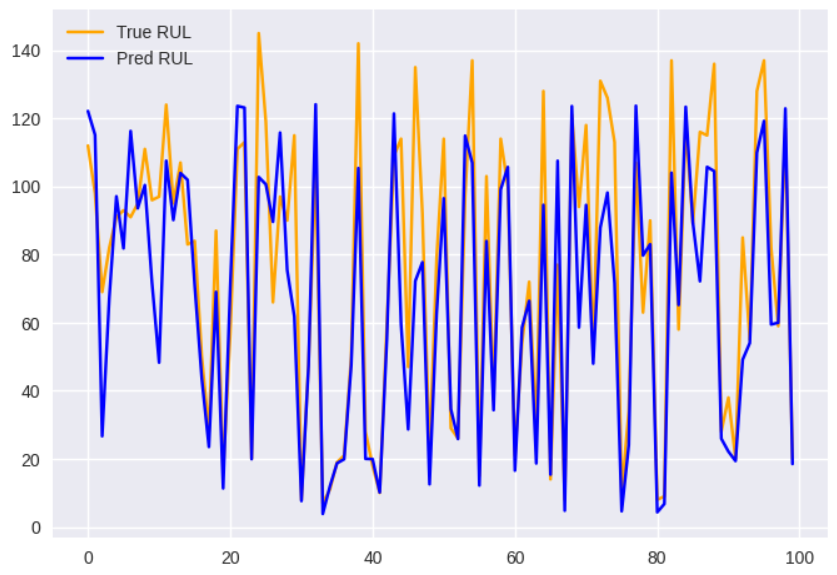
\includegraphics[width=0.92\textwidth]{images/pred_vs_actual_v3-plot.png}
	\caption{مقایسه مقادیر پیش‌بینی‌شده و واقعی RUL برای موتورهای آزمون}
	\label{fig:pred-vs-actual-final}
\end{figure}

قرار گرفتن بخش قابل توجهی از پیش‌بینی‌ها در پایین‌تر از مقادیر واقعی با هدف استفاده از تابع زیان نامتقارن سازگار است. در نتیجه، شکل حاصل علاوه بر آنکه عملکرد مدل را نمایش می‌دهد، رفتار طراحی‌شده آن را نیز آشکار می‌کند.

البته کم‌برآورد بیش از حد نیز می‌تواند هزینه عملیاتی ایجاد کند. اگر عمر موتور به صورت دائمی کمتر از مقدار واقعی برآورد شود، ممکن است بازرسی‌ها و تعمیرات غیرضروری افزایش یابند. بنابراین، هدف کاربردی یک سامانه صنعتی، دستیابی به کم‌برآورد حداکثری نیست؛ بلکه دستیابی به نقطه‌ای مناسب میان ایمنی، هزینه نگهداری و عدم‌قطعیت است. مقدار $\tau=0.125$ در این پژوهش به عنوان یک انتخاب اولیه و محافظه‌کارانه ارزیابی شده و نه به عنوان مقدار بهینه عمومی برای همه انواع موتورها. بنا به نوع و جنس موجودیت‌ها در لایه فیزیکی و میزان خسارتی که خرابی آن‌ها به بار می‌آورند، می‌توان ضریب $tau$ را تغییر داد.

\section{جایگاه مدل LSTM در معماری پیشنهادی}
\label{sec:lstm-role}

نتایج این بخش نشان می‌دهد که مدل LSTM انتخاب‌شده توانسته است یک سرویس پیش‌بینی قابل استفاده برای سامانه فراهم کند. با این ‌حال، لازم است جایگاه این نتیجه در کل پژوهش به‌درستی مشخص شود.

هدف پژوهش حاضر طراحی یک معماری جدید برای رقابت مستقیم با تمامی مدل‌های پیشرفته پیش‌بینی \gls{RUL} نیست. LSTM در اینجا به عنوان یک مدل تخصصی پیش‌بینی در عامل پیش‌بینی قرار گرفته است. این جداسازی از نظر معماری اهمیت دارد، زیرا مدل پیش‌بینی می‌تواند در آینده با مدل‌های دیگری جایگزین شود، بدون آنکه عامل دوقلو، عامل پایش، عامل زبانی یا واسط کاربر نیازمند بازطراحی اساسی باشند.

این ویژگی یکی از مزایای اصلی معماری چندعاملی است. در سیستم‌های چندعاملی، مسئولیت‌ها میان عامل‌های تخصصی توزیع می‌شوند و هر عامل می‌تواند وظیفه مشخصی را انجام دهد \cite{dorri2018multiagent,pretel2022masdt,lopez2024madtwin}. از این منظر، مدل LSTM بخشی از معماری است و نه خود معماری.


در مقایسه با این مسیر، سهم مدل پیش‌بینی حاضر در آن است که یک مدل نسبتاً ساده و قابل پیاده‌سازی را به عنوان جزء محاسباتی معماری چندعاملی به کار گرفته و خروجی آن را در یک زنجیره کامل داده، پیش‌بینی، پایش، توضیح و کنترل قرار داده است. همچنین استفاده واقعی در صنعت را نیز در نظر گرفته و نسبت کم‌برآورد‌ها را افزایش داده است.

\section{ارزیابی عامل تعامل زبانی}
\label{sec:llm-evaluation}

یکی از اهداف اصلی معماری پیشنهادی، ایجاد یک رابط طبیعی میان کاربر و دوقلوی دیجیتال است. همان‌طور که در فصل چهارم توضیح داده شد، عامل زبانی، خود وظیفه تولید مقدار \gls{RUL} را بر عهده ندارد؛ بلکه خروجی عددی عامل پیش‌بینی را دریافت کرده، وضعیت موتور را تفسیر کرده و در صورت نیاز فرمان مناسب را به عامل دوقلو ارسال می‌کند. این جداسازی برای جلوگیری از مخلوط شدن وظیفه استنتاج عددی با وظیفه تعامل انسانی اهمیت دارد.

برای ارزیابی عامل زبانی، شش فرایند کاربردی اجرا شده است. این فرایند‌ها شامل معرفی قابلیت‌های عامل، پرس‌وجوی وضعیت موتور سالم، پرس‌وجوی وضعیت موتور بحرانی، خاموش‌کردن همه موتورها، روشن‌کردن همه موتورها و خاموش‌کردن موتورهای در معرض خطر بوده‌اند.

\begin{table}[ht]
	\centering
	\caption{فرایند‌های ارزیابی عامل تعامل زبانی}
	\label{tab:llm-case-final}
	\begin{tabular}{p{0.6cm}p{3.3cm}p{5cm}p{3cm}}
		\toprule
		\textbf{\#} & \textbf{فرایند} & \textbf{هدف} & \textbf{نتیجه} \\
		\midrule
		۱ & معرفی عامل & بررسی دسترسی به قابلیت‌ها & صحیح \\
		۲ & پرس‌وجوی موتور سالم & دریافت و تفسیر \gls{RUL} & صحیح \\
		۳ & پرس‌وجوی موتور بحرانی & تشخیص وضعیت و ارائه دلیل & صحیح \\
		۴ & خاموش‌کردن همه موتورها & اجرای فرمان کنترلی & موفق \\
		۵ & روشن‌کردن همه موتورها & بازگرداندن وضعیت عملیاتی & موفق \\
		۶ & خاموش‌کردن موتورهای در خطر & ترکیب پیش‌بینی و کنترل & موفق \\
		\bottomrule
	\end{tabular}
\end{table}

در آزمایش انجام‌شده، ۳۰ درخواست مختلف برای عامل زبانی مورد بررسی قرار گرفته و نرخ موفقیت درخواست‌ها ۱۰۰ درصد گزارش شده است. منظور از موفقیت در اینجا، اجرای صحیح مسیر تعریف‌شده در گردش‌کار، دریافت داده مورد انتظار و تولید پاسخ یا اعمال فرمان مورد انتظار است؛ بنابراین این عدد نباید با معیارهایی مانند دقت مدل زبانی عمومی یا صحت آزاد و نامحدود استدلال مقایسه شود.

\subsection{تفسیر خروجی پیش‌بینی توسط عامل زبانی}

یکی از کاربردهای مهم عامل زبانی، تبدیل مقدار عددی \gls{RUL} به اطلاعات قابل فهم برای کاربر است. برای نمونه، در آزمایش انجام‌شده، مقدار \gls{RUL} موتور ۲ برابر ۶۳٫۷۷ چرخه و مقدار \gls{RUL} موتور ۲۴ برابر ۲۷٫۴۱ چرخه گزارش شده است. با توجه به آستانه تعریف‌شده، موتور ۲ در محدوده عادی و موتور ۲۴ در وضعیت بحرانی قرار گرفته است. تصاویر موجود در شکل‌های 
\ref{qa:llm-engine-query-2}
و
\ref{qa:llm-engine-query-24}
نمونه پرسیدن در باره موتور‌های ۲ و ۲۴ را از عامل زبانی می‌توان دید.

% \begin{figure}[H]
% 	\centering
% 	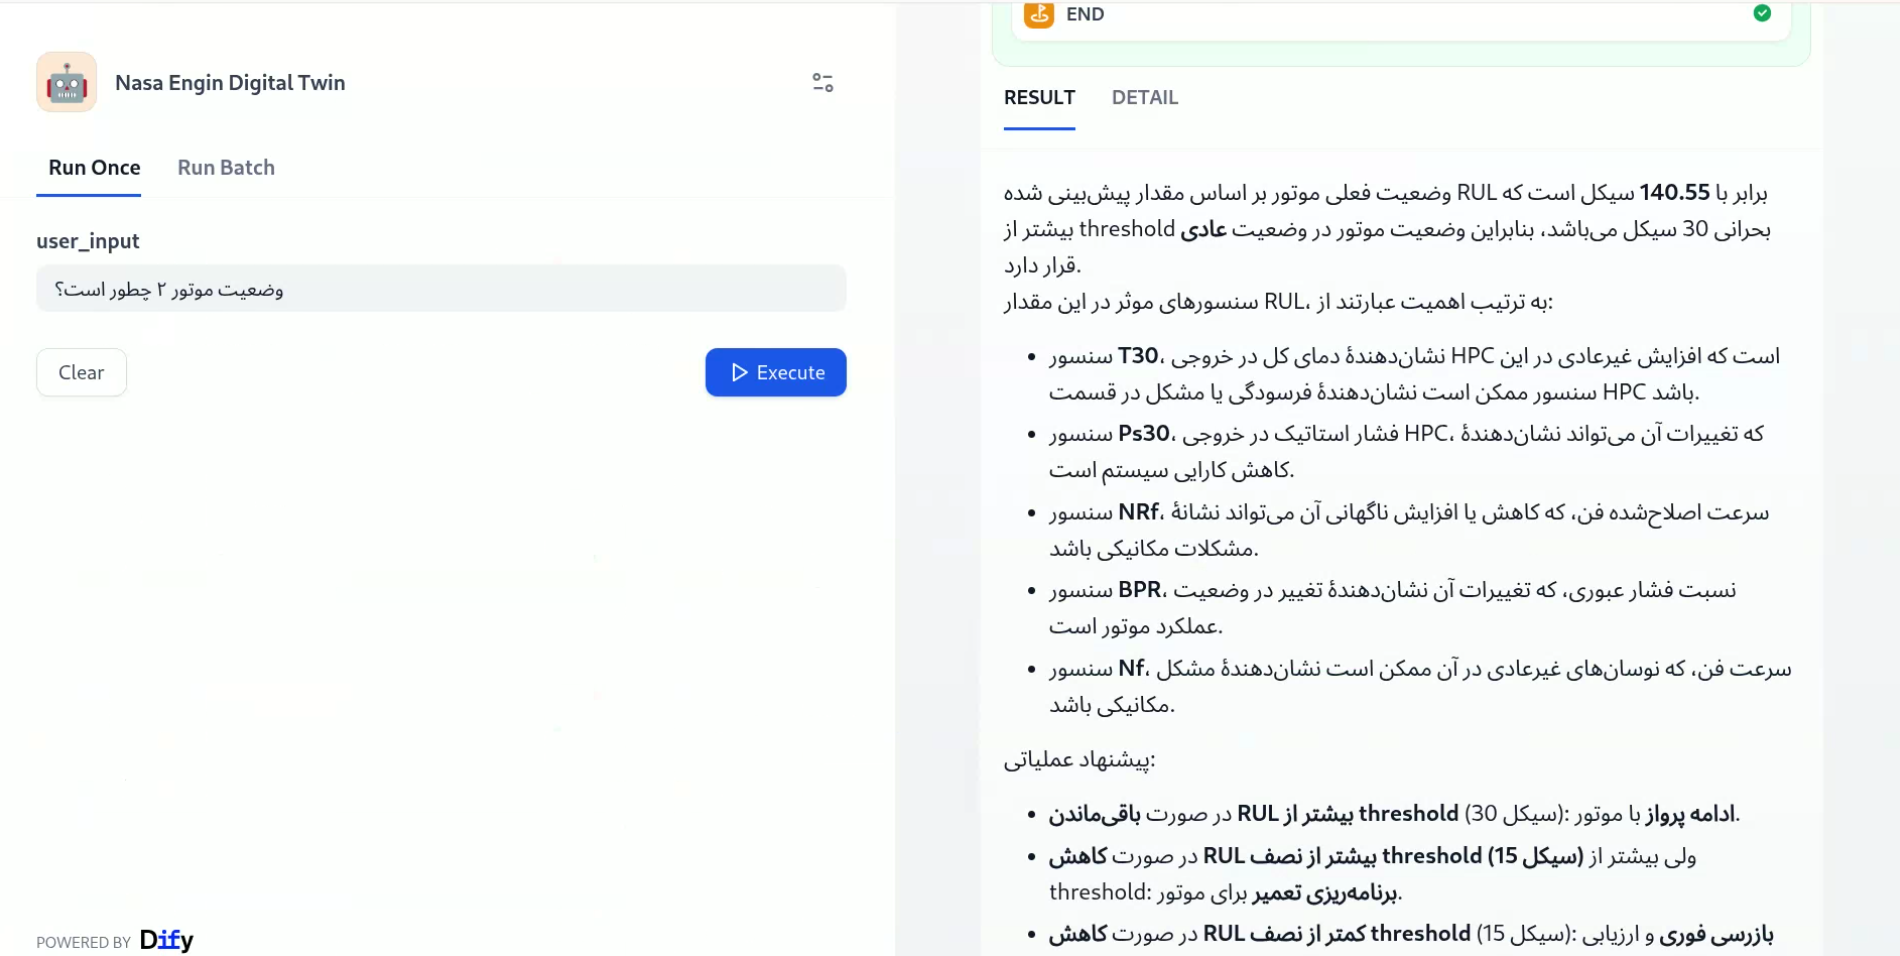
\includegraphics[width=0.95\textwidth]{images/llm_engine2_query.png}
% 	\caption{نمونه پاسخ عامل زبانی برای پرس‌وجوی وضعیت موتور ۲}
% 	\label{fig:llm-engine2-final}
% \end{figure}

% \begin{figure}[H]
% 	\centering
% 	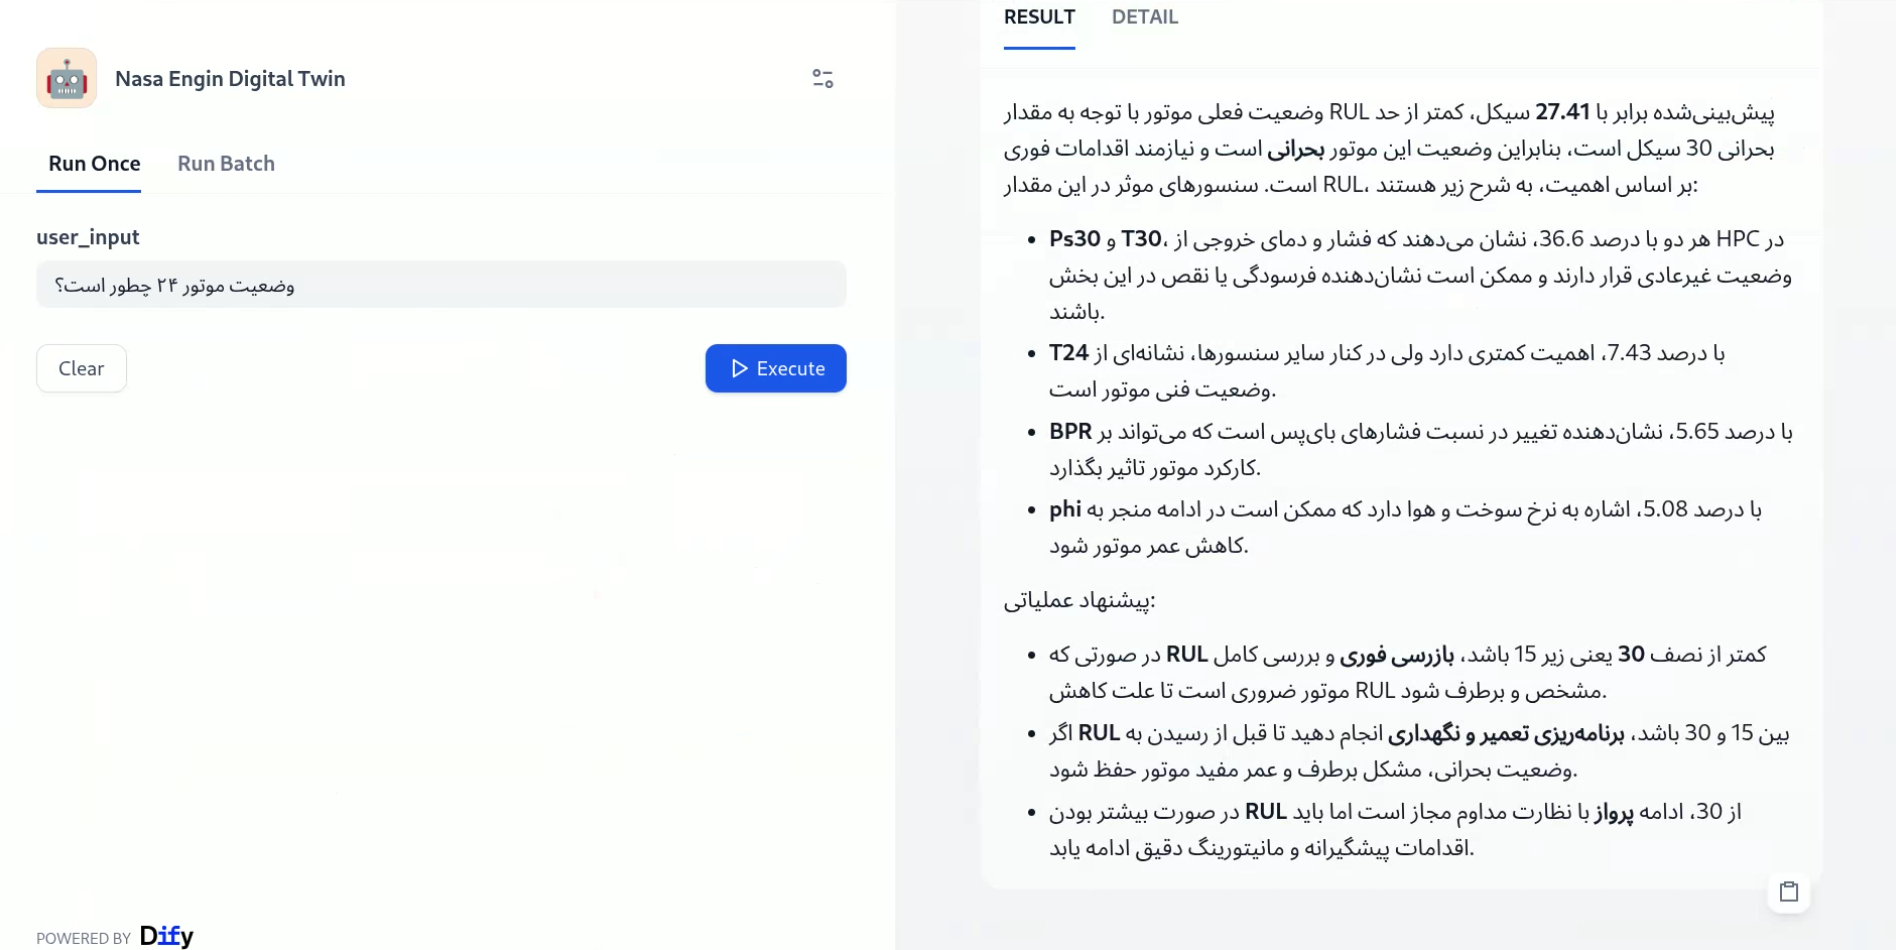
\includegraphics[width=0.95\textwidth]{images/llm_engine24_query.png}
% 	\caption{نمونه پاسخ عامل زبانی برای پرس‌وجوی وضعیت موتور ۲۴}
% 	\label{fig:llm-engine24-final}
% \end{figure}

نکته مهم آن است که عامل زبانی مقدار \gls{RUL} را به صورت مستقل محاسبه نمی‌کند. مقدار عددی از سرویس پیش‌بینی دریافت می‌شود و مدل زبانی بزرگ صرفاً وظیفه تفسیر و ارائه آن را بر عهده دارد. این معماری از نظر قابلیت اعتماد اهمیت دارد، زیرا محاسبه عددی در یک سرویس تخصصی و قابل ارزیابی باقی می‌ماند و مدل زبانی در نقش واسط و هماهنگ‌کننده قرار می‌گیرد.

در فرایند موتور ۲۴ نمایش داد شده در شکل 
\ref{qa:llm-engine-query-24}
، عامل زبانی علاوه بر بیان مقدار \gls{RUL}، مهم‌ترین حسگرهای مؤثر را نیز به کاربر معرفی کرده و برای هر یک تفسیری ارائه می‌دهد. این قابلیت، خروجی یک مدل عددی را به اطلاعاتی تبدیل می‌کند که برای کاربر نهایی قابل استفاده‌تر است.


\subsection{ارزیابی زمان پاسخ}

علاوه بر صحت مسیرهای عملیاتی، زمان پاسخ عامل زبانی نیز اندازه‌گیری شده است. برای ۳۰ درخواست بررسی‌شده، توزیع زمان پاسخ دارای دو ناحیه اصلی است.

\begin{figure}[H]
	\centering
	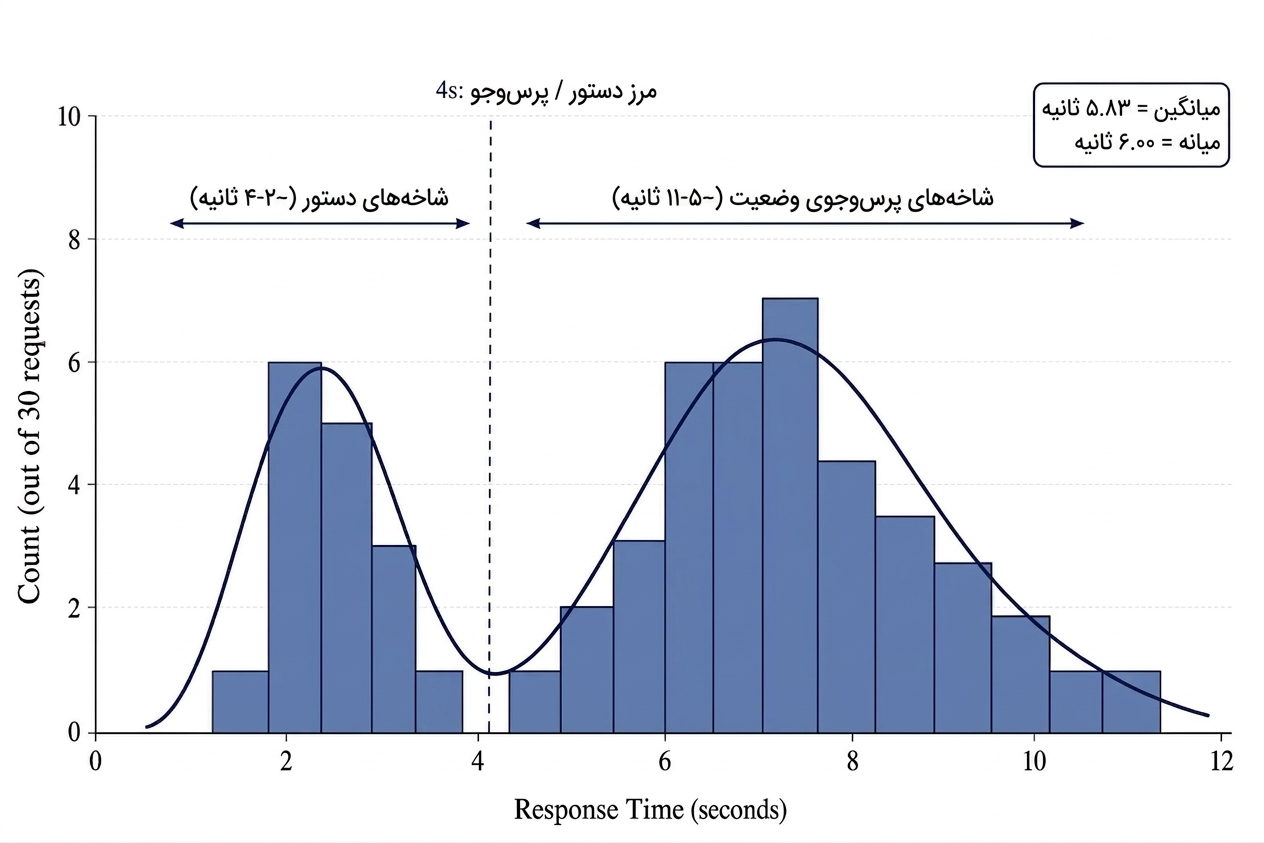
\includegraphics[width=0.90\textwidth]{images/latency_histogram2.png}
	\caption{توزیع زمان پاسخ عامل زبانی برای ۳۰ درخواست}
	\label{fig:latency-hist-final}
\end{figure}

با توجه به نمودار 
\ref{fig:latency-hist-final}،
بخش اول در حدود ۲ تا ۴ ثانیه مربوط به درخواست‌های ساده کنترلی است، درحالی‌که درخواست‌های مربوط به وضعیت موتور به دلیل طی‌کردن چند مرحله، زمان بیشتری نیاز دارند.

\begin{figure}[H]
	\centering
	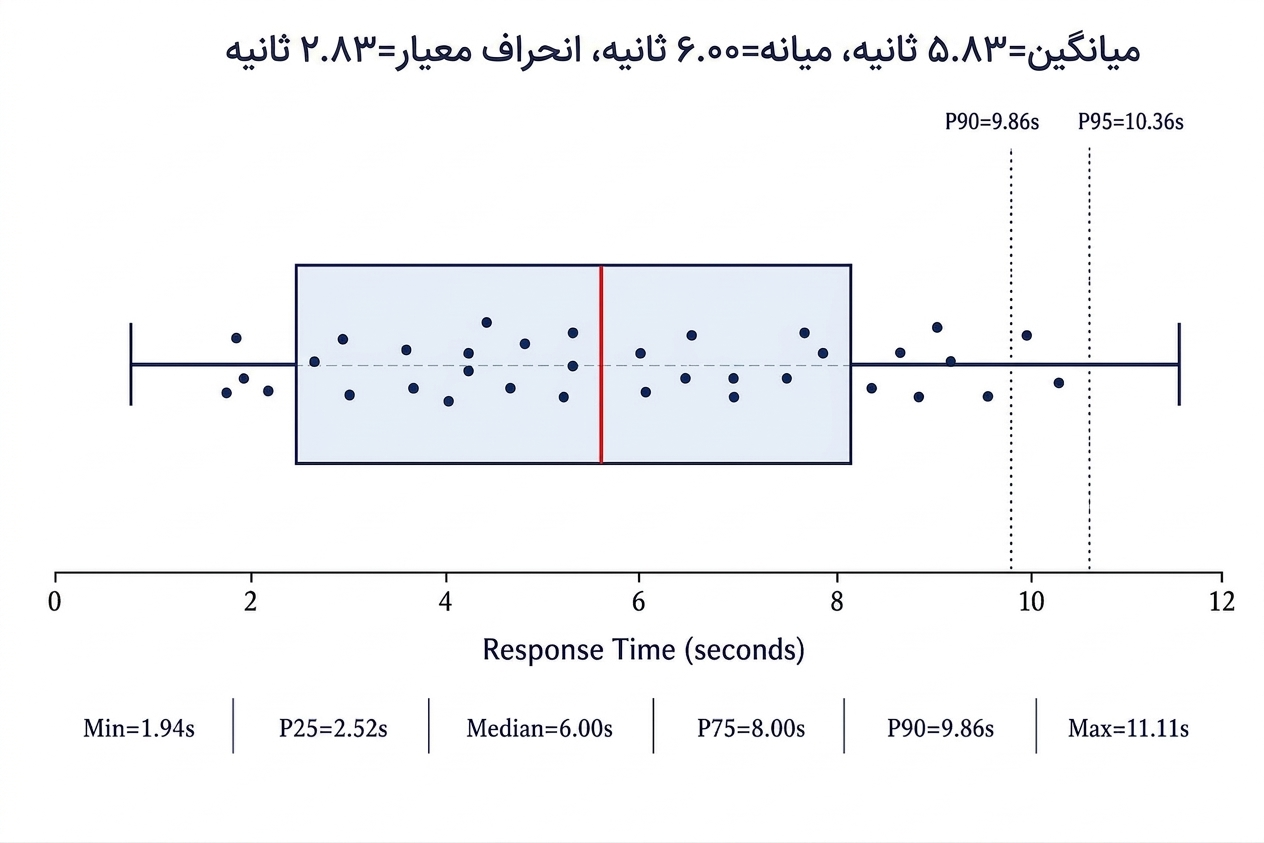
\includegraphics[width=0.90\textwidth]{images/latency_boxplot2.png}
	\caption{نمودار جعبه‌ای زمان پاسخ عامل زبانی}
	\label{fig:latency-box-final}
\end{figure}

در نمودار جعبه‌ای 
\ref{fig:latency-box-final}
نیز مشخص است  که
میانه زمان پاسخ حدود ۶ ثانیه و صدک نودم برابر ۹٫۸۶ ثانیه به دست آمده است. این مقدار برای نمونه آزمایشگاهی حاضر قابل قبول است، اما برای یک سامانه صنعتی بلادرنگ نمی‌توان صرفاً بر همین نتیجه تکیه کرد. کاهش وابستگی به API خارجی، استفاده از مدل‌های سبک‌تر، حافظه نهان، پردازش محلی و روش‌های رویدادمحور می‌توانند زمان پاسخ را کاهش دهند.

\section{ارزیابی پایش و حلقه بسته تصمیم}
\label{sec:closed-loop-evaluation}

مهم‌ترین تفاوت میان یک مدل پیش‌بینی مستقل و معماری پیشنهادی، در امکان تبدیل خروجی پیش‌بینی به یک جریان عملیاتی است. در فصل چهارم، این جریان در سطح پیاده‌سازی نشان داده شد. در این فصل، نتیجه آن از دیدگاه ارزیابی معماری بررسی می‌شود.

در فرایند نخست، کاربر درباره وضعیت یک موتور پرس‌وجو می‌کند. درخواست پس از تشخیص نیت، به عامل پیش‌بینی ارسال می‌شود و نتیجه به عامل زبانی بازمی‌گردد. عامل زبانی نتیجه را به شکل قابل فهم ارائه می‌کند.

در فرایند دوم، کاربر دستور می‌دهد موتورهای در معرض خطر خاموش شوند. در این حالت، مسیر به صورت جریان 
\ref{eq:flow}
طی می‌شود.

\begin{equation}
	\label{eq:flow}
	\text{پیش‌بینی}
	\rightarrow
	\text{تصمیم}
	\rightarrow
	\text{کنترل}
	\rightarrow
	\text{به‌روزرسانی وضعیت}
	\rightarrow
	\text{مشاهده وضعیت}
\end{equation}


این حلقه نشان می‌دهد که دوقلوی دیجیتال در پیاده‌سازی حاضر تنها یک مخزن اطلاعات نیست. تغییر وضعیت ایجادشده توسط فرمان نیز به دوقلو بازمی‌گردد و در نمایش پایش قابل مشاهده می‌شود. چنین ویژگی‌ای با مفهوم دوقلوی دیجیتال به عنوان یک سیستم پویا و متصل به موجودیت متناظر سازگارتر است \cite{tao2018digital,qi2021enabling}.

\begin{figure}[H]
	\centering
	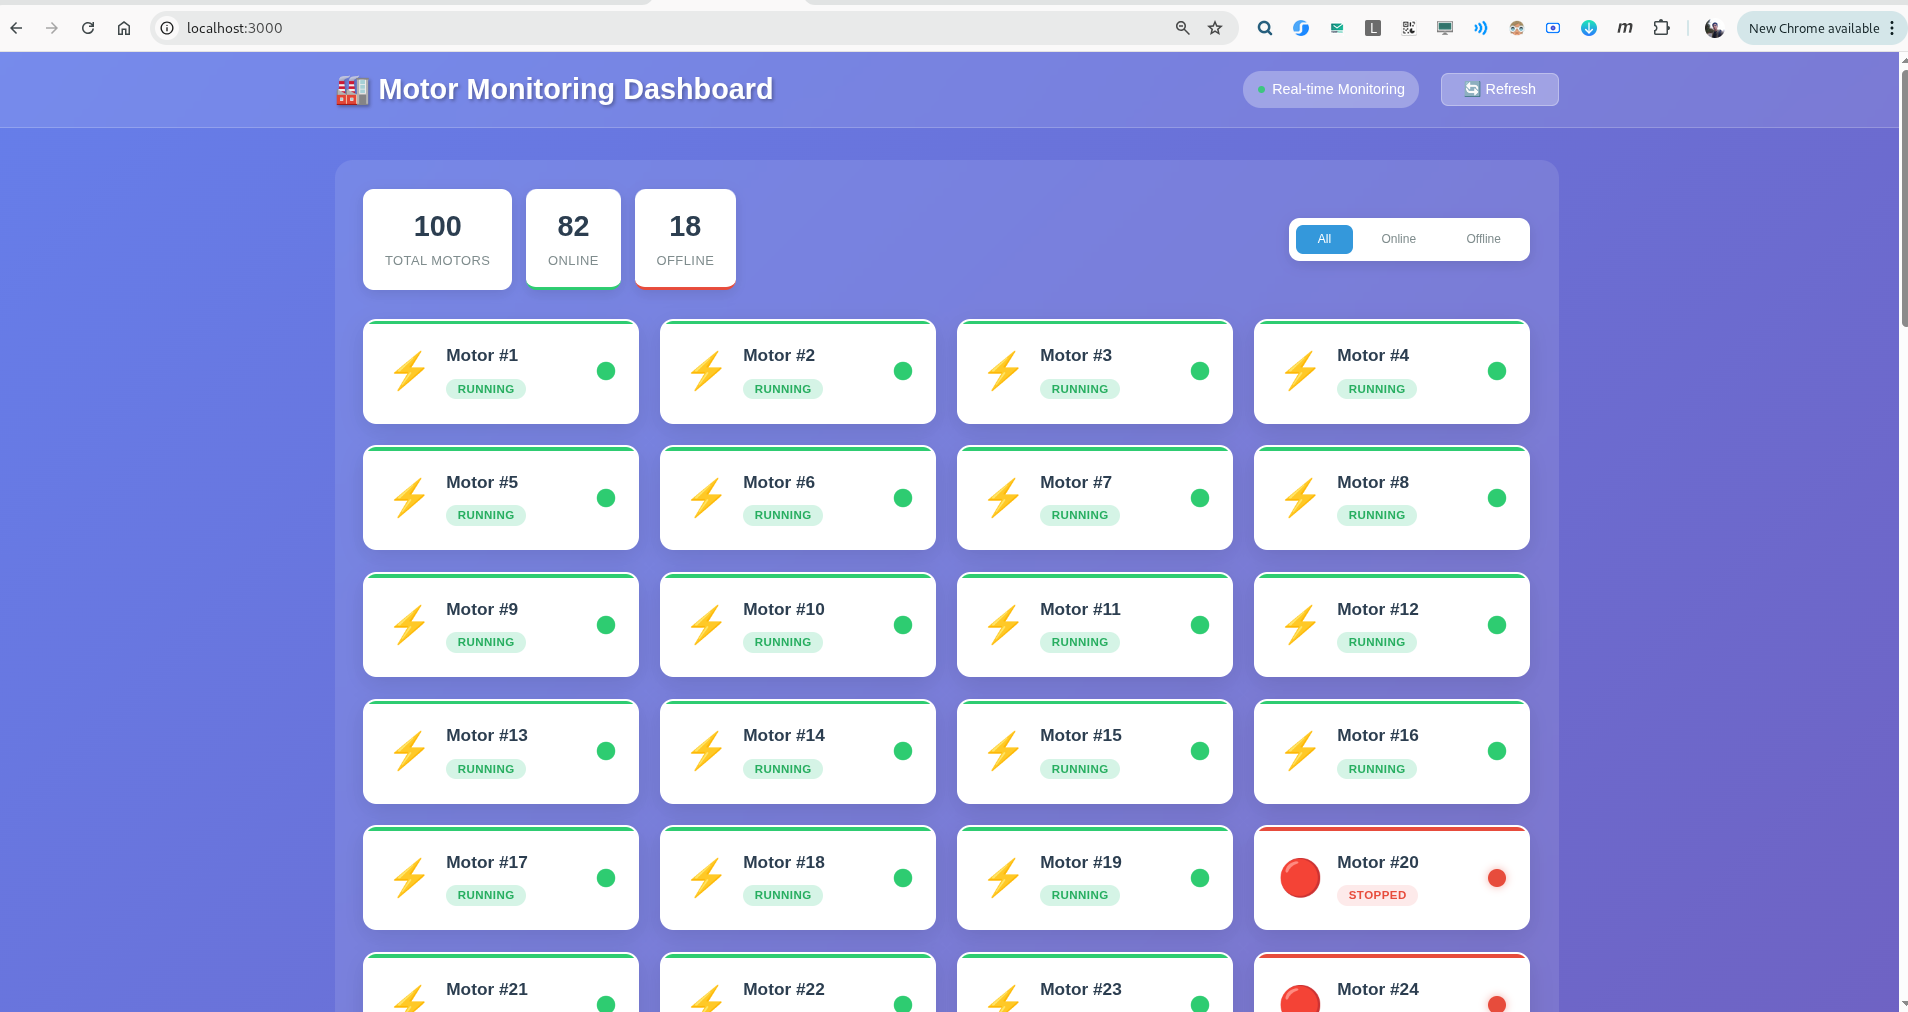
\includegraphics[width=0.90\textwidth]{images/monitor_after_critical_off.png}
	\caption{رابط پایش پس از اجرای فرمان خاموش‌سازی موتورهای در معرض خطر}
	\label{fig:closed-loop-final}
\end{figure}

از منظر معماری، این آزمایش اهمیت بیشتری از یک پاسخ موفق مدل زبانی بزرگ دارد؛ زیرا نشان می‌دهد چند سرویس مستقل توانسته‌اند یک فرایند مشترک را تکمیل کنند. عامل پیش‌بینی بدون عامل دوقلو نمی‌تواند وضعیت عملیاتی را تغییر دهد، عامل زبانی بدون سرویس پیش‌بینی نمی‌تواند درباره \gls{RUL} پاسخ تخصصی ارائه کند و عامل پایش بدون دریافت خروجی پیش‌بینی قادر به تشخیص موتورهای کم‌عمر نیست. بنابراین، ارزش معماری دقیقاً در تعامل این اجزا آشکار می‌شود.




% -----------------------------------------------------------------------
\section{مقایسه با پژوهش‌های مرتبط}
\label{sec:comparison}

هدف از این بخش، مشخص کردن جایگاه پژوهش حاضر نسبت به پژوهش‌هایی است که هر یک بخشی از مسئله مورد نظر این پژوهش را بررسی کرده‌اند. از این رو، چند پژوهش پایه از حوزه‌های دوقلوهای دیجیتال، سیستم‌های چندعاملی، نگهداری پیش‌بینانه و مدل‌های زبانی بزرگ انتخاب شده‌اند و قابلیت‌های آن‌ها در کنار قابلیت‌های چارچوب پیشنهادی مقایسه می‌شود.

موهانراج
 و
بالاجی
در سال ۲۰۲۶ در یک مرور جامع، روند توسعه فناوری
دوقلوهای دیجیتال، معماری‌ها، کاربردها، روش‌های مدل‌سازی و چالش‌های
یکپارچه‌سازی آن با فناوری‌هایی مانند هوش مصنوعی و اینترنت اشیاء را
بررسی کرده‌اند \cite{mohanraj2026digitaltwin}. یکی از نکات مهم این
مطالعه، تأکید بر ضرورت حرکت دوقلوهای دیجیتال از یک نمایش مجازی ساده به
سمت سامانه‌هایی یکپارچه، داده‌محور و هوشمند است. همچنین موضوعاتی مانند
مقیاس‌پذیری، قابلیت همکاری و یکپارچه‌سازی اجزای مختلف به عنوان مسائل
مهم توسعه دوقلوهای دیجیتال آینده مطرح شده‌اند. پژوهش حاضر این دیدگاه
را در سطح پیاده‌سازی دنبال می‌کند. به این صورت که دوقلوی دیجیتال،
عامل پایش، عامل پیش‌بینی و عامل مدل زبانی به صورت اجزای مستقل در یک معماری واحد قرار گرفته‌اند. بنابراین، سهم پژوهش حاضر
در این بخش، تبدیل قابلیت‌های عمومی مطرح‌شده در مطالعه‌ی مروری به یک
نمونه اجرایی قابل آزمایش است.

در حوزه ترکیب سیستم‌های چندعاملی و دوقلوهای دیجیتال،
کولیبالی
و
هملیش
در سال ۲۰۲۶ یک مرور نظام‌مند بر بیش از ۵۴۷ پژوهش انجام داده‌اند
و ضمن ارائه طبقه‌بندی معماری‌های ترکیبی، چالش‌های موجود در کاربرد
دوقلوهای دیجیتال چندعاملی برای نگهداری پیش‌بینانه را بررسی کرده‌اند
\cite{coulibaly2026madtdt}. اهمیت این پژوهش برای پژوهش حاضر
بیش از یک مطالعه مروری معمولی است، زیرا نویسندگان سه مسئله باز را به
عنوان مسیرهای اصلی پژوهش آینده مطرح می‌کنند که یکی از مسئله‌ها، سازمان‌دهی سلسله‌مراتبی دوقلوهای دیجیتال برای کنترل هوشمند که در آن برآورد عمر مفید باقیمانده و هوش مصنوعی توضیح‌پذیر نیز در نظر گرفته شود.

این مسئله مطرح‌شده توسط کولیبالی و هملیش ارتباط مستقیمی با جایگاه
پژوهش حاضر دارد. در آن مقاله بیان می‌شود که هنوز سامانه‌ای که بتواند
دوقلوهای دیجیتال، هماهنگی عامل‌ها، برآورد عمر مفید باقیمانده و
توضیح‌پذیری را در یک راهکار یکپارچه و سلسله‌مراتبی برای کاربردهای
صنعتی ترکیب کند، به طور کامل ارائه نشده است
\cite{coulibaly2026madtdt}. پژوهش حاضر بخشی از این خلأ را در یک
نمونه اجرایی مشخص پوشش می‌دهد. در این پژوهش، عامل پیش‌بینی \gls{RUL} در
کنار عامل دوقلوی دیجیتال و سایر عامل‌های کاربردی قرار گرفته و خروجی
پیش‌بینی نیز مستقیماً در اختیار عامل مدل زبانی قرار می‌گیرد. به این
ترتیب، نتیجه پیش‌بینی تنها یک مقدار عددی نیست، بلکه می‌تواند از طریق زبان طبیعی برای کاربر توضیح داده شود و بر اساس شرایط موتور، پیشنهاد عملی ارائه کند. بنابراین، پژوهش حاضر می‌تواند یک نمونه عملی از این مسئله باز را ارائه دهد و به عنوان یک گام اجرایی در راستای پرسش باز این مقاله در نظر گرفته شود.

از سوی دیگر، پژوهش کولیبالی و هملیش عمدتاً بر طبقه‌بندی معماری‌ها،
فناوری‌ها و چالش‌های موجود تمرکز دارد و هدف آن ارائه یک پیاده‌سازی
موردی برای یک تجهیز مشخص نیست. در پژوهش حاضر، مفاهیم مطرح‌شده به یک معماری عملیاتی تبدیل شده‌اند. به گونه‌ای که هر قابلیت
اصلی در قالب یک عامل مستقل قابل توسعه قرار گرفته است. این ویژگی باعث
می‌شود عامل پیش‌بینی بتواند در آینده با مدل دیگری جایگزین شود، بدون
آنکه الزاماً عامل دوقلو یا عامل زبان طبیعی تغییر کند. از این منظر،
چند عاملی بودن معماری پیشنهادی، پاسخی عملی به نیاز مطرح‌شده در مطالعات
جدید برای ایجاد معماری‌های انعطاف‌پذیر و قابل توسعه است.

در حوزه استفاده از مدل‌های زبانی بزرگ،
 فن و همکاران در سال ۲۰۲۶
چارچوبی برای استفاده از مدل زبانی بزرگ در محیط‌های صنعتی مبتنی بر
دوقلوی دیجیتال ارائه کرده‌اند که در آن مدل‌های زبانی بزرگ در فرآیند تصمیم‌گیری و
یادگیری تقویتی مورد استفاده قرار می‌گیرد \cite{fan2026llmrl}. این
پژوهش نشان می‌دهد که مدل‌های زبانی بزرگ می‌توانند دوقلوی دیجیتال را از یک محیط
صرفاً شبیه‌سازی و تحلیل به محیطی برای تصمیم‌گیری هوشمند تبدیل کنند.
با این حال، تمرکز آن بر هدایت فرآیند یادگیری تقویتی است. در حالی که
در پژوهش حاضر مدل زبانی بزرگ در نقش واسط شناختی و تعاملی میان کاربر و دوقلوی
دیجیتال قرار می‌گیرد. عامل زبان طبیعی می‌تواند وضعیت موتور را
بازیابی کند، درباره مقدار \gls{RUL} پرس‌وجو کند، دلیل وضعیت پیش‌بینی‌شده را
بر اساس اطلاعات موجود توضیح دهد و در صورت تعریف دستورات مجاز، فرمان
عملیاتی را به عامل مربوطه منتقل کند.

این تفاوت با جهت‌گیری پژوهش‌های جدید در زمینه عامل‌های هوشمند نیز
هم‌راستا است.
 حسن
 و 
 نگوین
 در سال ۲۰۲۶ بر ترکیب عامل‌های هوشمند و
دوقلوهای دیجیتال برای ایجاد سامانه‌های تصمیم‌گیری هوشمند تأکید
کرده‌اند \cite{hasan2026agenticdt}. در چنین رویکردهایی، دوقلوی دیجیتال
می‌تواند به عنوان منبع وضعیت سامانه و عامل هوشمند به عنوان لایه
استدلال و تصمیم‌گیری عمل کند. پژوهش حاضر این ایده را به یک فرایند
نگهداری پیش‌بینانه منتقل کرده است. به این صورت که عامل زبانی نه
جایگزین دوقلوی دیجیتال یا مدل پیش‌بینی، بلکه به عنوان یک لایه تعامل
روی آن‌ها قرار می‌گیرد. بنابراین، خروجی عددی مدل یادگیری عمیق به
اطلاعات قابل استفاده برای کاربر تبدیل می‌شود.

در بخش پیش‌بینی، پژوهش‌های مبتنی بر مجموعه داده \gls{CMAPSS} عمدتاً
با هدف کاهش خطای پیش‌بینی \gls{RUL} و توسعه معماری‌های یادگیری عمیق انجام
شده‌اند. در پژوهش حاضر نیز \lr{LSTM} به عنوان مدل پایه پیش‌بینی استفاده
شده است؛ با این تفاوت که هدف پژوهش، ارائه بهترین مدل پیش‌بینی برای
\lr{CMAPSS}
 نیست. 
 \lr{LSTM} 
در اینجا یک مؤلفه قابل تعویض در معماری است که وظیفه
فراهم کردن سرویس تخمین \gls{RUL} را بر عهده دارد. از این رو، امکان جایگزینی
آن با مدل‌های دیگر در آینده وجود دارد، بدون آنکه ساختار کلی دوقلوی
دیجیتال چندعاملی نیازمند بازطراحی اساسی باشد.

تفاوت مهم دیگر در نحوه استفاده از خروجی مدل پیش‌بینی است. در بسیاری
از پژوهش‌های \lr{CMAPSS}، خروجی اصلی مدل یک مقدار \gls{RUL} یا مجموعه‌ای از
معیارهای خطای پیش‌بینی است و ارزیابی عمدتاً در سطح مدل انجام می‌شود.
در پژوهش حاضر، این مقدار بخشی از وضعیت دوقلوی دیجیتال محسوب شده و
می‌تواند در اختیار عامل‌های دیگر قرار گیرد. علاوه بر این، تابع زیان
با توجه به اهمیت عملی خطای بیش‌برآورد \gls{RUL} طراحی شده است تا در شرایط
خطا، پیش‌بینی بیش از حد خوش‌بینانه نسبت به وضعیت واقعی موتور تا حد
امکان کاهش یابد. این انتخاب با هدف استفاده صنعتی از سامانه انجام شده
است، زیرا در نگهداری پیش‌بینانه، پیامدهای یک پیش‌بینی بیش از حد
خوش‌بینانه می‌تواند از یک پیش‌بینی محافظه‌کارانه بسیار پر هزینه‌‌تر باشد.

برآیند این مطالعات نشان می‌دهد که هر یک از پژوهش‌های پایه بخش مهمی
از چارچوب مورد نیاز را پوشش داده‌اند، اما تمرکز آن‌ها متفاوت است.
مقایسه قابلیت‌های اصلی در جدول \ref{tab:comparison-capabilities}
ارائه شده است.

\begin{table}[ht]
	\centering
	\caption{مقایسه قابلیت‌های پژوهش حاضر با پژوهش‌های پایه}
	\label{tab:comparison-capabilities}
	\resizebox{\textwidth}{!}{
		\begin{tabular}{p{4.4cm}ccccc}
			\toprule
			\textbf{قابلیت} &
			\textbf{موهانراج و بالاجی (۲۰۲۶)} &
			\textbf{کولیبالی و هملیش (۲۰۲۶)} &
			\textbf{فن و همکاران (۲۰۲۶)} &
			\textbf{حسن و نگوین (۲۰۲۶)} &
			
			\textbf{پژوهش حاضر} \\
			\midrule
			دوقلوی دیجیتال &
			\checkmark & \checkmark & \checkmark & \checkmark & \textbf{\checkmark} \\
			سیستم چندعاملی &
			-- & \checkmark & محدود & \checkmark & \textbf{\checkmark} \\
			معماری ماژولار و عامل‌های مستقل &
			محدود & \checkmark & محدود & \checkmark & \textbf{\checkmark} \\
			پیش‌بینی RUL &
			محدود & \checkmark & -- & -- & \textbf{\checkmark} \\
			استفاده از LSTM &
			-- & -- & -- & -- & \textbf{\checkmark} \\
			استفاده از CMAPSS &
			-- & -- & -- & -- & \textbf{\checkmark} \\
			کاهش هدفمند بیش‌برآورد RUL &
			-- & مطرح‌شده & -- & -- & \textbf{\checkmark} \\
			پایش وضعیت تجهیز &
			\checkmark & \checkmark & \checkmark & \checkmark & \textbf{\checkmark} \\
			دوقلوی دیجیتال دوطرفه در نمونه اجرایی &
			محدود & مطرح‌شده & محدود & محدود & \textbf{\checkmark} \\
			ادغام LLM با DT &
			-- & -- & \checkmark & \checkmark & \textbf{\checkmark} \\
			تعامل با زبان طبیعی &
			-- & -- & \checkmark & \checkmark & \textbf{\checkmark} \\
			توضیح خروجی پیش‌بینی برای کاربر &
			-- & \textbf{هدف آینده} & محدود & محدود & \textbf{\checkmark} \\
			ارائه پیشنهاد به کاربر &
			-- & \textbf{هدف آینده} & محدود & محدود & \textbf{\checkmark} \\
			نمونه اجرایی CMAPSS + MA-DT + LSTM + LLM &
			-- & -- & -- & -- & \textbf{\checkmark} \\
			\bottomrule
	\end{tabular}}
\end{table}

جدول \ref{tab:comparison-capabilities} نشان می‌دهد که پژوهش حاضر
در یک ویژگی منفرد لزوماً جایگزین پژوهش‌های پیشین نیست، بلکه قابلیت‌هایی
را که پیش‌تر عمدتاً به صورت جداگانه بررسی شده‌اند، در یک معماری واحد
به یکدیگر متصل می‌کند. این موضوع به ویژه در ارتباط با یافته‌های
\lr{Coulibaly}
و
\lr{Hamlich} 
 اهمیت دارد؛ زیرا مسئله‌ای که آن‌ها در سطح مرور
ادبیات به عنوان یک پرسش باز مطرح کرده‌اند، یعنی ترکیب دوقلوی دیجیتال،
هماهنگی عامل‌ها، برآورد \gls{RUL} و توضیح‌پذیری، در پژوهش حاضر در سطح یک
نمونه اجرایی مشخص دنبال شده است.

بنابراین، جایگاه پژوهش حاضر را می‌توان ایجاد یک پل میان چهار مسیر
اصلی پژوهش دانست. دوقلوی دیجیتال برای نمایش و همگام‌سازی وضعیت
موجودیت، سیستم چندعاملی برای تفکیک و مدیریت خدمات، یادگیری عمیق برای
تخمین \gls{RUL} و مدل زبانی بزرگ برای تعامل، توضیح و تصمیم‌یار. مزیت این ترکیب در اجزای مستقل و قابل تعویض آن است؛ به گونه‌ای که مدل پیش‌بینی، روش تعامل کاربر یا حتی نوع موجودیت فیزیکی می‌تواند در آینده تغییر کند، بدون آنکه اصل معماری نیازمند تغییر اساسی باشد.




\section{مزیت‌های معماری پیشنهادی}
\label{sec:architecture-benefits}

مهم‌ترین مزیت پژوهش حاضر را می‌توان در ترکیب چند قابلیت در یک معماری واحد دانست. هر یک از فناوری‌های استفاده‌شده پیش از این به صورت مستقل در پژوهش‌های مختلف بررسی شده‌اند، اما معماری حاضر تلاش می‌کند آن‌ها را در قالب یک زنجیره عملیاتی منسجم کنار یکدیگر قرار دهد.

نخستین مزیت، \textbf{جداسازی مسئولیت‌ها} است. عامل دوقلو، عامل پیش‌بینی، عامل پایش و عامل زبانی وظایف متفاوتی دارند. این جداسازی امکان جایگزینی هر جزء را بدون بازطراحی کل سامانه فراهم می‌کند.

دومین مزیت، \textbf{قابلیت توسعه} است. برای نمونه، می‌توان مدل LSTM را با مدل دیگری جایگزین کرد، بدون آنکه عامل زبانی یا رابط پایش تغییر اساسی کند.

سومین مزیت، \textbf{قابلیت تعامل طبیعی} است. کاربر برای دریافت وضعیت موتور مجبور نیست مستقیماً API یا ساختار داده را بشناسد و می‌تواند درخواست خود را به زبان طبیعی بیان کند.

چهارمین مزیت، \textbf{قابلیت اقدام} است. عامل زبانی صرفاً وضعیت را توضیح نمی‌دهد، بلکه در چارچوب فرمان‌های تعریف‌شده می‌تواند درخواست تغییر وضعیت را به دوقلوی دیجیتال منتقل کند.

پنجمین مزیت، \textbf{توجه به هزینه نامتقارن خطا} است. مدل پیش‌بینی با هدف یک کاربرد نگهداری، طراحی شده است و صرفاً به کمینه‌سازی خطا محدود نیست.

ششمین مزیت، \textbf{قابلیت توضیح خروجی} است. ترکیب وزن‌های توجه، داده حسگرها و عامل زبانی امکان ارائه توضیحی قابل فهم‌تر از یک مقدار عددی خام را فراهم کرده است.

هفتمین مزیت، \textbf{قابلیت انتقال معماری} است. از آنجا که ارتباط میان عامل‌ها از طریق سرویس‌ها و قراردادهای مشخص انجام می‌شود، می‌توان در آینده منبع داده یا مدل پیش‌بینی را تغییر داد.




\section{محدودیت‌های پژوهش}
\label{sec:limitations-final}

با وجود نتایج به‌دست‌آمده، برای جلوگیری از تعمیم بیش از حد یافته‌ها، محدودیت‌های پژوهش باید به‌صورت صریح بیان شوند.

نخستین محدودیت به مجموعه داده مربوط است. آزمایش کمی تنها روی \lr{FD001} انجام شده است. این زیرمجموعه یک شرایط عملیاتی و یک حالت خرابی دارد و بنابراین نمی‌توان نتایج حاصل را مستقیماً به \lr{FD002} تا \lr{FD004} یا شرایط واقعی عملیاتی تعمیم داد.

دومین محدودیت، مصنوعی بودن داده‌ها است. اگرچه \gls{CMAPSS} یکی از مجموعه داده‌های استاندارد و پرکاربرد در پژوهش‌های نگهداری پیش‌بینانه است، داده‌های آن جایگزین داده‌های حسگر واقعی موتور در حال بهره‌برداری نیستند. بنابراین، سامانه حاضر باید به عنوان یک نمونه آزمایشگاهی و اثبات امکان‌پذیری معماری تفسیر شود، نه یک سامانه آماده بهره‌برداری روی موتور واقعی.

سومین محدودیت، شبه‌بی‌درنگ بودن داده‌ها است. داده‌ها از فایل‌های CMAPSS استخراج و با پیشرفت ساعت شبیه‌سازی وارد سامانه شده‌اند. بنابراین، عملکرد واقعی شبکه حسگر، تأخیر ارتباطی، خرابی حسگر و نویز محیط واقعی در این آزمایش ارزیابی نشده است.

چهارمین محدودیت، نگهداری وضعیت در حافظه است. وضعیت ON/OFF موتور در نمونه فعلی پایدار نیست و با راه‌اندازی مجدد کانتینر از بین می‌رود. برای محیط صنعتی باید از پایگاه داده پایدار یا سامانه‌های مدیریت وضعیت توزیع‌شده استفاده شود.

پنجمین محدودیت، وابستگی عامل زبانی به سرویس بیرونی است. زمان پاسخ و هزینه فراخوانی مدل زبانی در مقیاس صنعتی می‌تواند اهمیت زیادی پیدا کند.

ششمین محدودیت، استفاده از آستانه‌های ثابت است. آستانه‌های وضعیت موتور در نسخه فعلی ثابت هستند، درحالی‌که یک سامانه صنعتی می‌تواند به آستانه‌های وابسته به شرایط عملیاتی، نوع موتور و وضعیت تاریخی تجهیز نیاز داشته باشد.

هفتمین محدودیت، نبود ارزیابی رسمی متخصصان حوزه هوافضا برای توضیحات تولیدشده توسط مدل زبانی بزرگ است. پاسخ‌های تولیدشده در این پژوهش از نظر ساختاری و عملکردی بررسی شده‌اند، اما اعتبار فیزیکی همه توضیحات حسگری باید در آینده توسط متخصصان موتور و نگهداری ارزیابی شود.



\section{جمع‌بندی}
\label{sec:chapter5-summary}
در این فصل، عملکرد سامانه پیشنهادی از دو منظر مدل پیش‌بینی و معماری چندعاملی ارزیابی شد تا مشخص شود آیا چارچوب ارائه‌شده توانایی تبدیل یک مدل پیش‌بینی عمر مفید باقیمانده به بخشی از یک سامانه یکپارچه برای پایش، تفسیر و تصمیم‌گیری را دارد یا خیر. ارزیابی کمی مدل پیش‌بینی بر روی زیرمجموعه \lr{FD001} از مجموعه داده \gls{CMAPSS} انجام شد و عملکرد مدل \lr{LSTM-MSE} و مدل \lr{LSTM-Pinball} با استفاده از معیارهای \lr{MAE}، \lr{RMSE}، $R^2$ و نسبت کم‌برآورد مورد مقایسه قرار گرفت. نتایج نشان داد که مدل \lr{LSTM-Pinball} با استفاده و تابع زیان \lr{Pinball} با $\tau=0.125$ توانسته است نسبت کم‌برآورد را از ۰٫۵۲ در مدل \lr{LSTM-MSE} به ۰٫۷۱ در مدل نهایی افزایش دهد. این تغییر در نسبت کم‌برآورد به عنوان یک ویژگی طراحی‌شده و مرتبط با هدف ایجاد رفتار محافظه‌کارانه در پیش‌بینی تفسیر شد، نه صرفاً به عنوان یک بهبود عمومی در دقت مدل. در عین حال، نتایج نشان دادند که این انتخاب نباید به معنای تلاش برای بیشینه‌سازی کم‌برآورد تلقی شود، زیرا کم‌برآورد بیش از حد نیز می‌تواند به افزایش بازرسی‌ها و اقدامات نگهداری غیرضروری منجر شود. از این رو، مقدار $\tau=0.125$ در این پژوهش به عنوان یک انتخاب اولیه و محافظه‌کارانه برای قرار دادن مدل در زنجیره تصمیم‌گیری در نظر گرفته شده است.

از منظر معماری، نتایج نشان داد که مدل \lr{LSTM} به عنوان یک مؤلفه تخصصی و قابل تعویض، توانسته است سرویس پیش‌بینی مورد نیاز معماری را فراهم کند، بدون آنکه مدل پیش‌بینی به هسته اصلی معماری وابسته باشد. این موضوع با هدف کلی پژوهش سازگار است، زیرا مسئله اصلی پژوهش رقابت میان مدل‌های مختلف یادگیری عمیق برای دستیابی به کمترین خطای ممکن روی \gls{CMAPSS} نبوده است؛ بلکه هدف، قرار دادن یک مدل پیش‌بینی قابل قبول درون یک معماری چندعاملی بوده است. بنابراین، نتایج مدل باید در ارتباط با نقش آن در کل سامانه تفسیر شوند و نه به عنوان ادعایی درباره برتری عمومی \lr{LSTM} یا مدل lr{LSTM-Pinball} نسبت به تمامی روش‌های موجود.

در ادامه، عامل تعامل زبانی از نظر قابلیت اجرای فرایندهای تعریف‌شده، تفسیر خروجی پیش‌بینی و زمان پاسخ مورد بررسی قرار گرفت. در ۳۰ درخواست آزمایش‌شده، نرخ موفقیت فرایندهای تعریف‌شده ۱۰۰ درصد به دست آمد. این ارزیابی نشان داد که عامل زبانی می‌تواند مقدار \gls{RUL} دریافت‌شده از سرویس پیش‌بینی را به اطلاعات قابل فهم برای کاربر تبدیل کند. همچنین می‌تواند وضعیت موتور را بر اساس آستانه‌های تعریف‌شده تفسیر نماید و در چارچوب فرمان‌های مجاز، درخواست‌های کنترلی را به عامل دوقلوی دیجیتال منتقل کند.علاوه‌ بر این اندازه‌گیری زمان پاسخ نشان داد که میانه زمان پاسخ حدود ۶ ثانیه و صدک نودم برابر با ۹٫۸۶ ثانیه بوده است. این زمان برای نمونه آزمایشگاهی حاضر قابل قبول ارزیابی شد، اما به دلیل وابستگی به سرویس بیرونی و تفاوت میان محیط آزمایشگاهی و محیط صنعتی، نمی‌توان آن را به عنوان تضمین عملکرد بلادرنگ در کاربردهای صنعتی در نظر گرفت.

مهم‌ترین یافته معماری در ارزیابی، حلقه بسته تصمیم است. در این فرایند، خروجی پیش‌بینی به تصمیم‌گیری منتقل شده، تصمیم به فرمان کنترلی تبدیل گردیده، وضعیت دوقلوی دیجیتال به‌روزرسانی شده و نتیجه تغییر وضعیت در لایه پایش قابل مشاهده بوده است. در نتیجه، دوقلوی دیجیتال در نمونه پیاده‌سازی‌شده صرفاً به عنوان یک مخزن اطلاعاتی مورد استفاده قرار نگرفته، بلکه در یک چرخه عملیاتی میان داده، پیش‌بینی، تصمیم، کنترل و بازخورد قرار گرفته است. این ویژگی نشان می‌دهد که ارزش معماری پیشنهادی تنها در عملکرد مستقل هر عامل نیست، بلکه در نحوه همکاری عامل‌های تخصصی برای تکمیل یک فرایند سرتاسری نمایان می‌شود.

مقایسه با پژوهش‌های مرتبط نیز نشان داد که پژوهش حاضر در یک قابلیت منفرد لزوماً جایگزین مطالعات پیشین نیست، بلکه تلاش می‌کند چند مسیر پژوهشی شامل دوقلوهای دیجیتال، سیستم‌های چندعاملی، پیش‌بینی \gls{RUL}، پایش و مدل‌های زبان بزرگ را در قالب یک نمونه اجرایی واحد به یکدیگر متصل کند. جداسازی مسئولیت‌ها میان عامل دوقلوی دیجیتال، عامل پیش‌بینی، عامل پایش و عامل زبان طبیعی، امکان توسعه و جایگزینی مستقل اجزای سامانه را فراهم می‌کند و در عین حال، استفاده از مدل زبانی را از محاسبه مستقیم مقدار \gls{RUL} جدا نگه می‌دارد. بر این اساس، مهم‌ترین نتیجه فصل حاضر آن است که معماری پیشنهادی توانسته است یک مدل پیش‌بینی را از یک مؤلفه مستقل محاسباتی به بخشی از یک زنجیره عملیاتی شامل پیش‌بینی، تفسیر، تصمیم، کنترل و بازخورد تبدیل کند.

در نهایت، محدودیت‌های ارزیابی نیز باید در تفسیر این نتایج مورد توجه قرار گیرند. آزمایش کمی مدل تنها بر روی زیرمجموعه \lr{FD001} مجموعه داده \gls{CMAPSS} انجام شده و جریان داده به صورت شبه‌بی‌درنگ شبیه‌سازی شده است. همچنین وضعیت عملیاتی موتور در نمونه فعلی در یک زیرساخت پایدار ذخیره نمی‌شود و عامل زبان طبیعی به یک سرویس بیرونی وابسته است. بنابراین، نتایج این فصل را باید در چارچوب یک نمونه آزمایشگاهی و اثبات امکان‌پذیری معماری تفسیر کرد. با وجود این محدودیت‌ها، مجموعه آزمایش‌های انجام‌شده نشان می‌دهد که اجزای اصلی معماری پیشنهادی توانسته‌اند در کنار یکدیگر یک جریان عملیاتی منسجم ایجاد کنند و مبنای مناسبی برای جمع‌بندی نهایی پژوهش و بررسی دستاوردها و مسیرهای توسعه آینده فراهم آورند.



% \section{پیشنهادهایی برای کارهای آینده}
% \label{sec:future-work-final}

% مسیرهای آینده پژوهش را می‌توان در چهار دسته اصلی تقسیم کرد.

% در دسته نخست، باید دامنه داده گسترش یابد. آزمایش روی \lr{FD002} تا \lr{FD004} می‌تواند میزان مقاومت مدل و معماری را در برابر شرایط عملیاتی مختلف مشخص کند. همچنین استفاده از داده‌های واقعی حسگرهای موتور می‌تواند فاصله میان نمونه آزمایشگاهی و کاربرد صنعتی را کاهش دهد.

% در دسته دوم، مدل پیش‌بینی می‌تواند از یک مدل نقطه‌ای به سمت مدل‌های احتمالاتی حرکت کند. ترکیب \lr{LSTM} با سایر مدل‌های احتمالاتی و استفاده از مدل‌های دقیق‌تر با خطای کم‌تر می‌تواند در دقت خروجی مدل کمک کند و در نتیجه خروجی زبان طبیعی را نیز واضح‌تر کند.

% در دسته سوم، عامل زبانی می‌تواند با حافظه بلندمدت، پایگاه دانش فنی و دانش‌نگار حوزه هوافضا ترکیب شود. در این صورت، پاسخ عامل تنها بر اساس مقدار فعلی \gls{RUL} نخواهد بود، بلکه تاریخچه موتور، تعمیرات قبلی، شرایط عملیاتی و سوابق خرابی را نیز در نظر خواهد گرفت.

% در دسته چهارم، معماری می‌تواند به حوزه‌های دیگر منتقل شود. برای مثال، در یک کارخانه تولیدی، عامل دوقلو می‌تواند نماینده یک دستگاه \lr{CNC} باشد؛ عامل پیش‌بینی وضعیت خرابی دستگاه را تخمین بزند؛ عامل پایش وضعیت خط تولید را بررسی کند و عامل زبانی امکان پرس‌وجو و اجرای فرمان را فراهم آورد. به همین ترتیب، معماری می‌تواند برای سایر صنایع مورد نیاز نیز توسعه یابد.

% برای نزدیک شدن به استقرار صنعتی نیز پیشنهاد می‌شود ارتباط سرویس‌ها از مدل نظرسنجی دوره‌ای به سازوکارهای رویدادمحور منتقل شود و وضعیت دوقلو در یک زیرساخت پایدار ذخیره گردد. همچنین لازم است سیاست‌های کنترل دسترسی، ثبت رویداد، تأیید انسانی فرمان‌های حساس و سازوکارهای ایمنی در لایه عامل زبانی اضافه شوند.




% \section{جمع‌بندی نهایی}
% \label{sec:final-summary}

% هدف اصلی این پژوهش طراحی و پیاده‌سازی یک چارچوب دوقلوهای دیجیتال چندعاملی برای پایش و پیش‌بینی عمر مفید موتورهای توربوفن و بررسی امکان تعامل طبیعی با این دوقلوها بود. در این راستا، یک معماری چندلایه طراحی و سپس با استفاده از مجموعه داده \gls{CMAPSS} در قالب یک نمونه آزمایشگاهی پیاده‌سازی شد.

% نتایج نشان داد که مدل LSTM مورد استفاده می‌تواند به عنوان یک مؤلفه پیش‌بینی قابل استفاده در معماری عمل کند. مدل نهایی با استفاده از سازوکار توجه و \gls{PinballLoss} توانست \lr{MAE} برابر ۱۷٫۲۱ و $R^2$ برابر ۰٫۷۱ را روی مجموعه آزمون به دست آورد. همچنین نسبت کم‌برآورد از ۴۷ درصد در مدل پایه به ۸۷ درصد افزایش یافت. اهمیت نتیجه دوم در این است که مدل به صورت هدفمند به سمت پیش‌بینی محافظه‌کارانه حرکت کرده است؛ رویکردی که با ماهیت ایمنی‌محور نگهداری موتورها سازگارتر است. بااین‌حال، این نتایج به معنای ارائه بهترین مدل برای CMAPSS نیست و مدل پیش‌بینی در این پژوهش صرفاً به عنوان یک مؤلفه تخصصی و قابل جایگزینی در معماری در نظر گرفته شده است.

% در سطح سامانه‌ای، عامل زبانی توانست اطلاعات عددی تولیدشده توسط عامل پیش‌بینی را به زبان طبیعی تفسیر کند، وضعیت موتور را توضیح دهد و در فرایند‌های تعریف‌شده، فرمان‌های کنترلی را به دوقلوی دیجیتال ارسال کند. بررسی ۳۰ درخواست، نرخ موفقیت ۱۰۰ درصدی را در فرایند‌های تعریف‌شده نشان داد. همچنین حلقه بسته میان پیش‌بینی، تصمیم، کنترل و بازخورد در فرایند‌های عملیاتی اجرا شد.

% از دیدگاه معماری، مهم‌ترین دستاورد پژوهش در کنار هم قرار دادن قابلیت‌هایی است که معمولاً به صورت جداگانه بررسی می‌شوند: دوقلوی دیجیتال، سیستم چندعاملی، پیش‌بینی \gls{RUL}، پایش شبه‌بی‌درنگ و تعامل مبتنی بر مدل‌های بزرگ زبانی. این ترکیب امکان تبدیل یک مدل پیش‌بینی منفرد به یک سامانه تصمیم‌یار تعاملی را فراهم می‌کند. در چنین ساختاری، مدل یادگیری عمیق صرفاً تولیدکننده یک عدد نیست، بلکه خروجی آن وارد زنجیره‌ای می‌شود که می‌تواند به تشخیص وضعیت، ارائه توضیح، تصمیم‌گیری و در نهایت اقدام منجر شود.

% از منظر کاربرد صنعتی، این پژوهش یک نمونه اثبات امکان‌پذیری ارائه می‌کند و نه یک محصول آماده بهره‌برداری. برای رسیدن به سطح صنعتی، اتصال به داده‌های واقعی حسگر، پایگاه داده پایدار، مدیریت عدم‌قطعیت، اعتبارسنجی متخصصان، کنترل دسترسی و سازوکار تأیید انسانی فرمان‌های حساس ضروری است. با وجود این محدودیت‌ها، ساختار معماری به گونه‌ای طراحی شده است که این اجزا بتوانند در مراحل بعدی بدون تغییر بنیادی در منطق کلی سامانه اضافه شوند.

% در نهایت، می‌توان نتیجه گرفت که ارزش اصلی چارچوب پیشنهادی در \textbf{ترکیب پیش‌بینی، دوقلوی دیجیتال، عامل‌های تخصصی و تعامل زبانی در یک حلقه عملیاتی واحد} است. این ویژگی، معماری را از یک سامانه صرفاً پیش‌بینی‌کننده به سمت یک چارچوب دوقلوی دیجیتال چندعاملی قابل توسعه هدایت می‌کند؛ چارچوبی که می‌تواند در آینده با جایگزینی منبع داده، مدل پیش‌بینی و دانش حوزه، برای سایر تجهیزات و صنایع نیز مورد استفاده قرار گیرد.



